\documentclass{article}
\usepackage{graphicx}
\usepackage{multicol} % use to multiple column in itemize
\usepackage{float}
\usepackage{setspace}
\usepackage{hyperref}
\setlength{\parskip}{0.5em}

\begin{document}

\title{Dimensionality Reduction}
% \author{Cong Cuong PHAM}

\maketitle

\begin{abstract}
This document introduces some fundamental notions of Dimensionality Reduction.
\end{abstract}

\subsection{Dimensionality Reduction (Unsupdervised)}
\par The goal of dimensionality reduction is to systematically and intelligently reduce the number of features considered in a dataset. Stated differently, trim the fat off. Often times, in one's eagerness to collect enough data for machine learning to be effective, you might add irrelevant features to your dataset. Bad features have the effect of hindering the machine learning process, and make your data harder to understand. Dimensionality reduction attempts to trim your dataset down to the bare essentials needed for decision-making.

\begin{figure}[H]
\centering
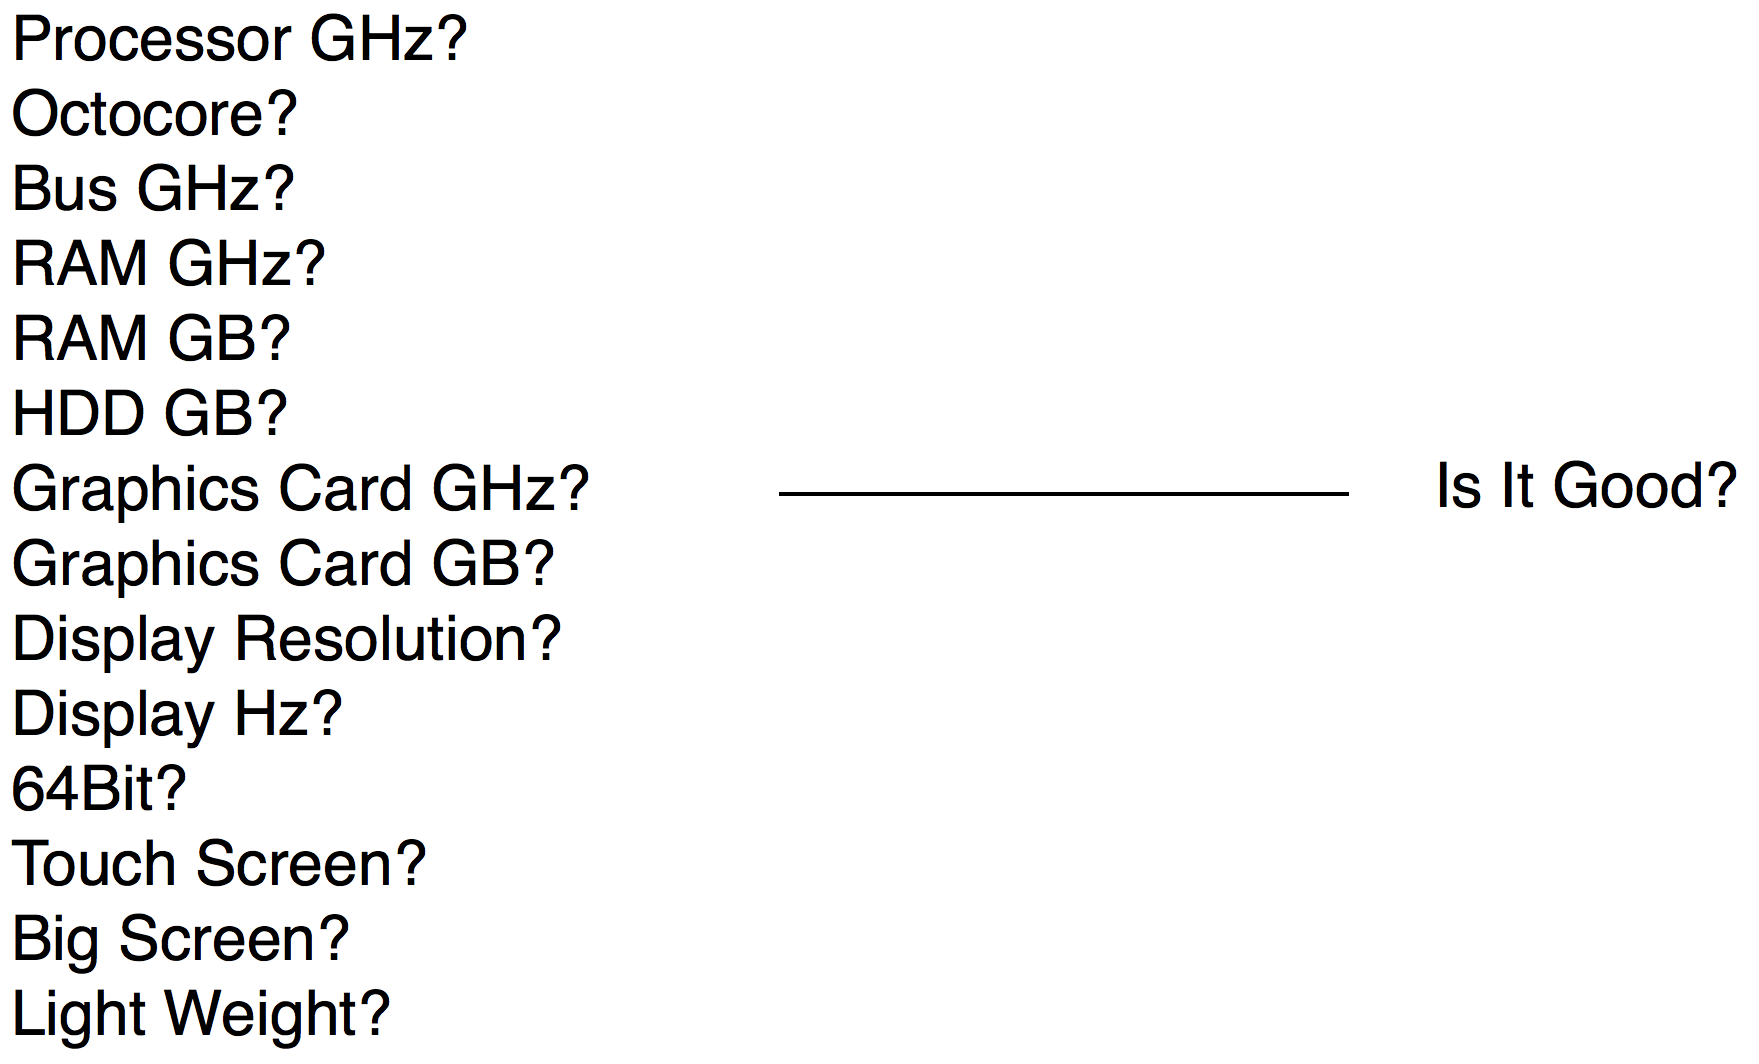
\includegraphics[width=0.6\linewidth]{pic/dimensionality-reduction.png}
\caption{Example of dimensionality reduction.}
\end{figure}

More examples

\begin{itemize}
    \item Given a 100 question survey, attempt to find the gist of what is truly being accessed; then rephrase it in just 5 questions.
    \item Build a robot that can recognize pictures of similar objects, even if they are rotated at odd angles and orientations.
    \item Compress a video stream by reducing the number of colors.
    \item Summarize a long book.
\end{itemize}

\par Dimensionality reduction falls into the realm of unsupervised learning because you don't instruct the computer which features you want it to build; the computer infers this information automatically by examining your unlabeled data.

\begin{flushright}
    source: \href{https://courses.edx.org/courses/course-v1:Microsoft+DAT210x+6T2016/courseware/e36e6b45ae5d4032bef2ec557c1ff48f/a8cf8333f6044e9b9a357b7797f282e3/?child=first}{course.edx.org}  
\end{flushright}
\end{document}